\documentclass{article}

% Language setting
% Replace `english' with e.g. `spanish' to change the document language
\usepackage[english]{babel}

% Set page size and margins
% Replace `letterpaper' with `a4paper' for UK/EU standard size
\usepackage[letterpaper,top=2cm,bottom=2cm,left=3cm,right=3cm,marginparwidth=1.75cm]{geometry}

% Useful packages
\usepackage{amsmath}
\usepackage{amsfonts}
\usepackage{graphicx}
\usepackage[colorlinks=true, allcolors=blue]{hyperref}

\usepackage{natbib}

\title{Evolutionary Pair HMM}
\author{Ian Holmes}

\begin{document}
%\maketitle

\section{Statistical alignment}

\subsection{General geometric indel model (GGI)}

A sequence $S(t)$ evolves by
substitutions (rate matrix $Q$),
deletions (rate $\mu$ per site, extension probability $y$),
and
insertions (rate $\lambda$, extension $x$,
characters drawn from $Q$'s stationary distribution $\pi$).

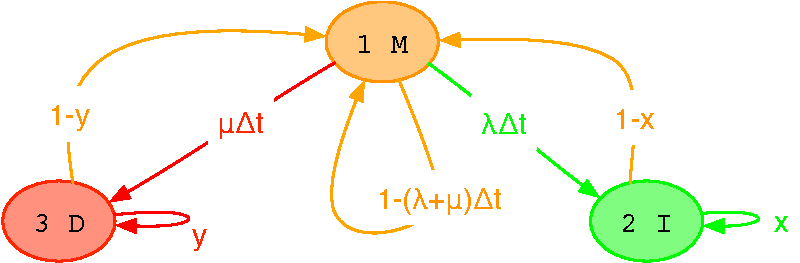
\includegraphics[width=\textwidth]{InstantHMM.pdf}

At equilibrium, sequence length $\sim$ Geometric($\lambda/\mu$). Composition is $\pi$.

If the model is required to be reversible then $\lambda y(1-x) = \mu x(1-y)$.

\subsection{Conditional Pair HMM (transducer) with time-varying parameters}
Derived in \cite{Holmes2020}.
A Pair HMM whose state path likelihood approximates $P(S(t)|S(0))$

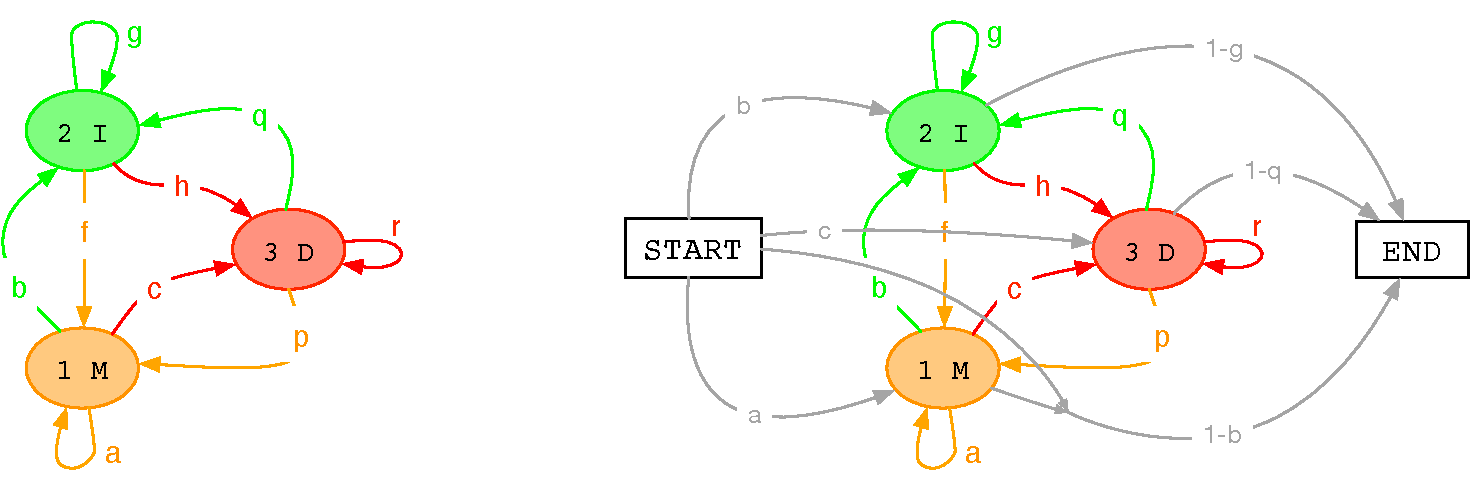
\includegraphics[width=\textwidth]{PairHMM.pdf}

At $t=0$: $a(0)=1$, $f(0)=1-x$, $g(0)=x$, $p(0)=1-y$, $r(0)=y$, and $b(0)=c(0)=h(0)=q(0)=0$.

For $t>0$, % following Holmes (2020)
\begin{eqnarray*}
\begin{bmatrix}
a & b & c \\
f & g & h \\
p & q & r 
\end{bmatrix}
& = &
\begin{bmatrix}
T_{MM} & T_{MI} & 1-T_{MM}-T_{MI} \\
T_{IM}/W_I & (W_I-T_{MI}-T_{DI})/W_I & (T_{MI}+T_{DI}-T_{IM})/W_I \\
(1-T_{MM}-T_{IM})/W_D & T_{DI}/W_D & (W_D+T_{MM}+T_{IM}-T_{DI}-1)/W_D 
\end{bmatrix}
\\
W_I(t) & = & \exp\left(\frac{\lambda t}{1-x}\right)-1 \\
W_D(t) & = & \exp\left(\frac{\mu t}{1-y}\right)-1 \\
T_{ij}(0) & = & \mbox{1 if $i=j=M$, 0 otherwise}
\\
  \frac{d}{dt} T_{MM}(t) & = &
  \mu \frac{b f (1-y)}{1 - g y}-(\lambda +\mu )a
  \nonumber \\
  \frac{d}{dt} T_{MI}(t) & = &
  -\mu \frac{b (1-g)}{1 - g y} + \lambda (1-b)
  \nonumber \\
  \frac{d}{dt} T_{IM}(t) & = &
  \lambda a - \mu \frac{f (1-g) (b (1-r)+c q)}{(1 - g y) (f (1-r)+h p)}
  \nonumber \\
  \frac{d}{dt} T_{DI}(t) & = &
  \mu \frac{(1-g) (b (1-r-h q)+c g q)}{(1-g y) (f (1-r)+h p)}
\end{eqnarray*}

The $T_{ij}(t)$ may be approximated by Runge-Kutta methods,
e.g. Dormand-Prince. % \cite{DormandPrince1980}

The substitution matrix for the M state of the Pair HMM is
the matrix exponential $\exp(Qt)$, for which a Pad\'{e} approximant
or other power series expansion can be used. % \cite{MolerVanLoan2003}

\subsection{Exactly-solved special case (TKF91)}

When $x=y=0$ the model is TKF91 \cite{ThorneEtAl91}
with solution
$
\begin{bmatrix}
a & b & c \\
f & g & h \\
p & q & r 
\end{bmatrix}
=
\begin{bmatrix}
(1-\beta)\alpha & \beta & (1-\beta)(1-\alpha) \\
(1-\beta)\alpha & \beta & (1-\beta)(1-\alpha) \\
(1-\gamma)\alpha & \gamma & (1-\gamma)(1-\alpha)
\end{bmatrix}
$
where
$\alpha = \exp(-\mu t)$,
$\beta = \frac{\lambda \left( \exp(-\lambda t) - \exp(-\mu t) \right)}{\mu \exp(-\lambda t) - \lambda \exp(-\mu t)}$
and
$\gamma = 1 - \frac{\mu \beta}{\lambda (1 - \alpha)}$.



\subsection{Alignment unspecified}

Suppose a prefix list (or tree) of sequences.
Node 1 corresponds to the empty sequence.
Nodes $N>1$ correspond to nonempty sequences $S_N$.
Character $\omega_N$ is the last character of $S_N$.
The parent node $\psi_N$ corresponds to the longest prefix of $S_N$:
removing $\omega_N$ from $S_N$ leaves $S_{\psi_N}$.

Let $F(i,j,t) = \begin{bmatrix} F_M & F_I & F_D \end{bmatrix}$
be the per-state Forward likelihoods for sequences $S_i,S_j$.

We seek $F^\ast(i,j,t) = P(S(t)=S_j|S(0)=S_i)$.
The Forward recursions are, for $i>1$ and $j>1$
\begin{eqnarray*}
F(1,1,t) & = & \begin{bmatrix} 1 & 0 & 0 \end{bmatrix}
\\
F(1,j,t) & = &
F(1,\psi_j,t) U_I(\omega_j,t)
\\
F(i,1,t) & = &
F(\psi_i,1,t) U_D(\omega_i,t)
\\
F(i,j,t) & = &
F(\psi_i,\psi_j,t) U_M(\omega_i,\omega_j,t)
+ F(i,\psi_j,t) U_I(\omega_j,t)
+ F(\psi_i,j,t) U_D(\omega_i,t)
\\
F^\ast(i,j,t) & = & F(i,j,t) \begin{bmatrix}
1-b(t) \\
1-g(t) \\
1-q(t) \end{bmatrix}
\\
U_M(\omega_i,\omega_j,t) & = &
\begin{bmatrix}
a(t) & 0 & 0 \\
f(t) & 0 & 0 \\
p(t) & 0 & 0 
\end{bmatrix}
\exp(Qt)_{\omega_i \omega_j}
\\
U_I(\omega_j,t) & = &
\begin{bmatrix}
0 & b(t) & 0 \\
0 & g(t) & 0 \\
0 & q(t) & 0 
\end{bmatrix}
\pi_{\omega_j}
\\
U_D(\omega_i,t) & = &
\begin{bmatrix}
0 & 0 & c(t) \\
0 & 0 & h(t) \\
0 & 0 & r(t) 
\end{bmatrix}
\end{eqnarray*}

The time complexity to compute the Forward likelihood is $O(L^2)$,
where $L$ is the sequence length.

\subsection{Alignment specified}

The pairwise alignment of ancestor $i$ and descendant $j$ can be summarized by two lists:
\begin{itemize}
    \item The list $A_M$ of pairs of aligned characters $(\omega,\omega')$ from ancestor $S(0)$ and descendant $S(t)$;
    \item The list $A_{ID}$ of pairs of unaligned gap sequences $(\delta,\delta')$ that were deleted and inserted in between.
\end{itemize}

The alignment probability, computable in time $O(L)$ (and in practice very fast), is
\[
P(A_M,A_{ID},S(t)|S(0)) =
\prod_{(\omega,\omega') \in A_M} \exp(Qt)_{\omega \omega'}
\prod_{(\delta,\delta') \in A_{ID}} G(|\delta|,|\delta'|,t)
\prod_{\omega'\in \delta'} \pi_{\omega'}
\]

where $G(i,j,t)$ is the probability that between the next pair of aligned characters in $S(0)$ and $S(t)$,
there were $i$ characters deleted from $S(0)$ 
and $j$ characters inserted into $S(t)$,
with no homology
\begin{eqnarray*}
G(0,0,t) & = & a \\
G(i,0,t) & = & cr^{i-1}p \\
G(0,j,t) & = & bg^{j-1}f \\
G(i,j,t) & = &
g^{j-1} r^{i-1}
\sum_{k=0}^{\min(i,j)}
\left(\frac{hq}{gr}\right)^k
\left[
\binom{i}{k} \binom{j-1}{k} brf
+ \binom{i-1}{k} \binom{j-1}{k} (bhp+cqf)
+ \binom{i-1}{k} \binom{j}{k} cgp
\right]
\end{eqnarray*}
% The unobserved index $k$ counts zig-zags on the Pair HMM state path
% ($D \to I \to D$ or $I \to D \to I$).

\subsection{Phylogenetic alignment}

Both forms of the pairwise likelihood (alignment specified, or unspecified) can be extended to multiple sequences on a phylogeny.
Upgrade $\exp(Qt)$ to Felsenstein pruning. % \cite{Felsenstein81}.

For the alignment-unspecified form, use automata composition to obtain $N$-sequence HMMs \cite{SilvestreRyanEtAl2020}.
The resulting Forward algorithm is $O(L^N)$.
To ameliorate this, discard all but a few representative sample paths \cite{WestessonEtAl2012},
or use MCMC \cite{RedelingsSuchard2007}.


\section{Hierarchical geometric indel model (HGI)}

Consider a version of the model where some of the elements of the evolving sequence can themselves be evolving subsequences, recursively nested inside the parent,
potentially with different evolutionary parameters: e.g. a low-indel hydrophobic region.
This induces a recursive structure, like a parse tree.

The grammar is over {\em characters}, {\em links}, and {\em zones}:
\begin{itemize}
\item A character ($\omega_k, \omega'_k$) is an evolving observed residue ($\omega, \omega'$) with a fixed hidden type ($k$).
\item A link ($L,L^x,L^y$) is an element of a sequence. It's either a character or a nested zone.
\item A zone ($Z,Z^x,Z^y$) is an evolving sequence of links.
\end{itemize}

There are $N_z$ types of zone and $N_k$ types of character.

In a zone of type $i$, the indel rates are $(\lambda_i,\mu_i)$.
The probability that a random link in this zone is another recursively nested zone is $\eta_i$.
If so, the probability that the nested zone is of type $j$ is $\tau_{ij}$.

If the link is not a nested zone, the probability that it is a character of type $k$ is $\sigma_{ik}$.
The rate matrix for type $k$ is $Q^{(k)}$ and the stationary distribution is $\pi^{(k)}$.

The equilibrium distribution over parse trees is a stochastic context-free grammar (SCFG)
\[
\begin{array}{rclll}
  Z_i & \to & L_i & Z_i & \lambda_i/\mu_i \\
        & | & \epsilon & & 1 - \lambda_i/\mu_i \\
  L_i & \to & \omega_k & & (1-\eta_i) \sigma_{ik} \pi^{(k)}_{\omega} \\
      & | & Z_j & & \eta_i \tau_{ij}
\end{array}
\]

The joint distribution $P(S(0),S(t))$ is the Inside likelihood of a Pair SCFG

\begin{tabular}{ll}
$\begin{array}{rclll}
  Z_i & \to & M_i & & 1 \\
  Z^x_i & \to & L^x_i & Z^x_i & \lambda_i/\mu_i \\
        & | & \epsilon & & 1 - \lambda_i/\mu_i \\
  Z^y_i & \to & L^y_i & Z^y_i & \lambda_i/\mu_i \\
        & | & \epsilon & & 1 - \lambda_i/\mu_i \\
  L_i & \to & \omega_k & \omega'_k & (1-\eta_i) \sigma_{ik} \pi^{(k)}_{\omega} \exp(Q^{(k)} t)_{\omega \omega'} \\
      & | & Z_j & & \eta_i \tau_{ij} \\
  L^x_i & \to & \omega_k & & (1-\eta_i) \sigma_{ik} \pi^{(k)}_{\omega} \\
      & | & Z^x_j & & \eta_i \tau_{ij} \\
  L^y_i & \to & \omega'_k & & (1-\eta_i) \sigma_{ik} \pi^{(k)}_{\omega'} \\
      & | & Z^y_j & & \eta_i \tau_{ij}
\end{array}$ & $\begin{array}{rclll}
  M_i & \to & L_i & M_i & (\lambda_i/\mu_i) a_i \\
      & | & L^y_i & I_i & b_i \\
      & | & L^x_i & D_i & (\lambda_i/\mu_i) c_i \\
      & | & \epsilon & & (1 - \lambda_i/\mu_i) (1-b_i) \\
  I_i & \to & L_i & M_i & (\lambda_i/\mu_i) f_i \\
      & | & L^y_i & I_i & g_i \\
      & | & L^x_i & D_i & (\lambda_i/\mu_i) h_i \\
      & | & \epsilon & & (1 - \lambda_i/\mu_i) (1-g_i) \\
  D_i & \to & L_i & M_i & (\lambda_i/\mu_i) p_i \\
      & | & L^y_i & I_i & q_i \\
      & | & L^x_i & D_i & (\lambda_i/\mu_i) r_i \\
      & | & \epsilon & & (1 - \lambda_i/\mu_i) (1-q_i)
\end{array}$
\end{tabular}

\bibliographystyle{unsrt}
\bibliography{references}


\end{document}
